%\usepackage{casouso_estilo}
%\chapter{An\'alisis y Dise\~no} % (fold)

El capítulo de diseño, está conformado por la especificación de cómo está conformado el protocolo criptográfico. Dicho capítulo contiene la especificación de la plataforma del protocolo, es decir, los recursos tanto de hardware como de software necesarios para poder desarrollar el proyecto con las herramientas tecnológicas necesarias. El capítulo muestra los modelos de entidades del protocolo, dichos modelos comprenden el modelo entidad relación que corresponde a la base de datos creada para la persistencia de los datos involucrados en el protocolo, y el diagrama de clases que brinda un bosquejo del funcionamiento e interacción de atributos y operaciones del protocolo. Por último, se muestra la descripción de todos los casos de uso que conforman al proyecto. 





%=======================================================================================================================================
\section{Especificación de Plataforma}


%\textbf{Servidor web}
%\begin{enumerate}
%\item \textbf{Hardware}
%\begin{itemize}
%\item Procesador: Intel Xeon 1220
%\item RAM: 4 GB DDR3 1600 MHz
%\end{itemize}
%\item \textbf{Software}
%\begin{itemize}
%\item Sistema operativo: Debian 8 Jessie 64 bits
%\item Servidor web: Apache 2
%\begin{itemize}
%\item Módulo PHP 5 con conector para MongoDB
%\end{itemize}
%\item Servidor de base de datos: MongoDB 3.2
%\end{itemize}
%\item \textbf{Red}
%\begin{itemize}
%\item Conexión a internet cableada de 20 Mb/s
%\end{itemize}
%\end{enumerate}

\textbf{Estación de trabajo y computadores personales}
\begin{enumerate}
\item \textbf{Hardware}
\begin{itemize}
\item Procesador: Intel Core i3 o superior.
\item RAM: 2 GB o superior
\end{itemize}
\item \textbf{Software}
\begin{itemize}
\item Visual Paradigm Community Edition 13.2.
\item ArgoUML 0.34.
\item Inkscape 0.92.
\item Python 3.6.1.
\item Photoshop Online.
\item LaTeX.
\item MySQL Community Edition.
\item MySQL Workbench.
\item ownCloud.
\end{itemize}
\item \textbf{Red}
\begin{itemize}
\item Conexión a internet de 2 Mb/s
\end{itemize}
\end{enumerate}

%=======================================================================================================================================
\section{Casos de Uso}

\begin{figure}[htbp!]
\centering
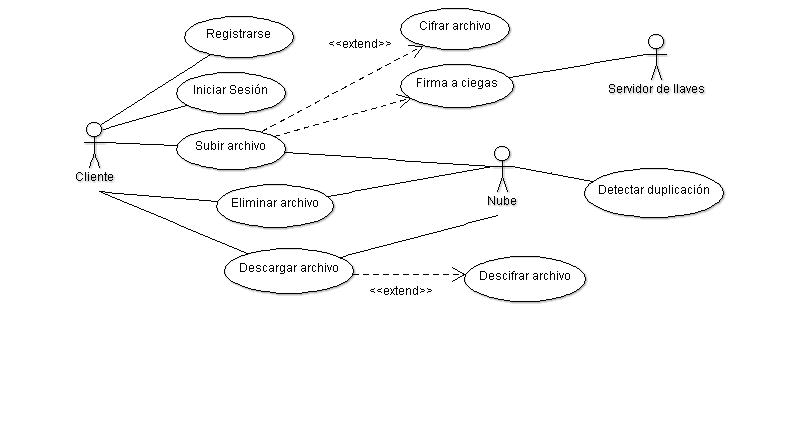
\includegraphics[width=1\textwidth]{images/CasosDeUso}
\caption{Diagrama de Casos de Uso del sistema.}
\end{figure}

\cfinput{casosUso/Servidor/CUSLLIndex}
\cfinput{casosUso/Nube/CUNIndex}
\cfinput{casosUso/Cliente/CUCLIndex}
\newpage
%=======================================================================================================================================
\section{Diagramas de secuencia}

\subsection{Registrar Usuario}

\begin{figure}[htbp!]
\centering
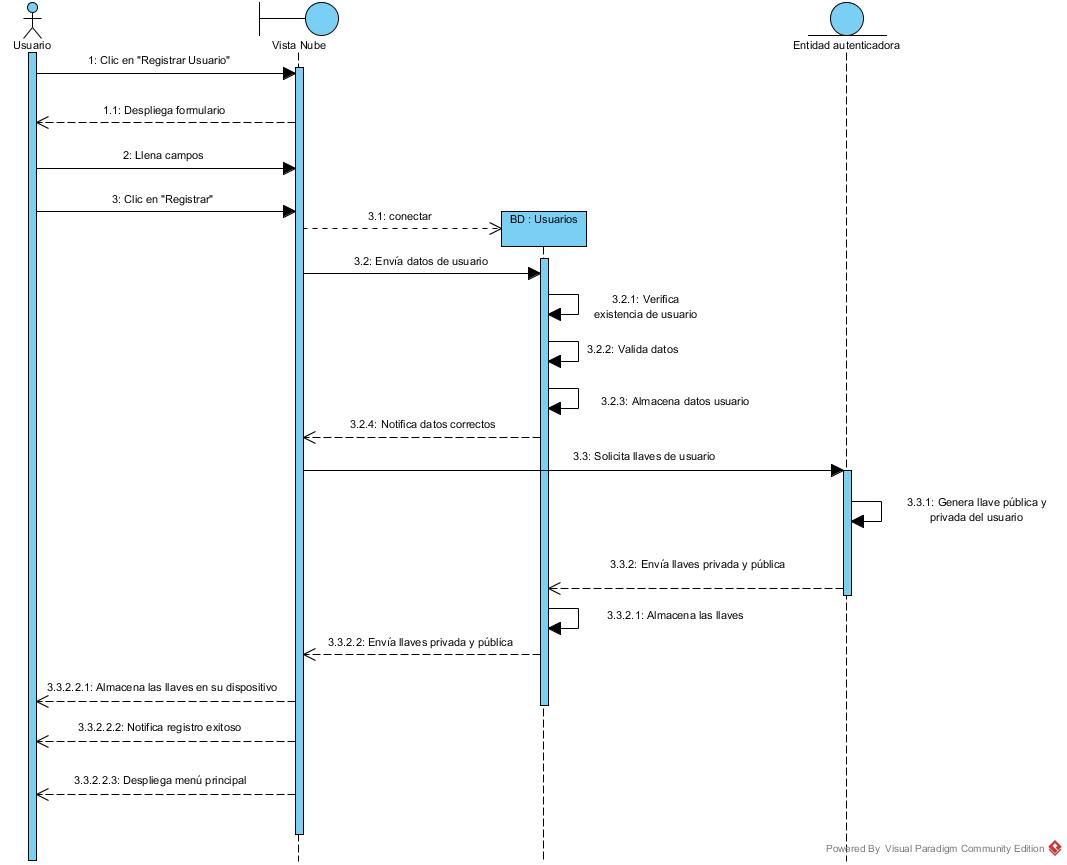
\includegraphics[width=1\textwidth]{images/Registrar_usuario}
\caption{Diagrama de secuencias de Registrar un usuario nuevo.}
\end{figure}

\begin{figure}[htbp!]
\centering
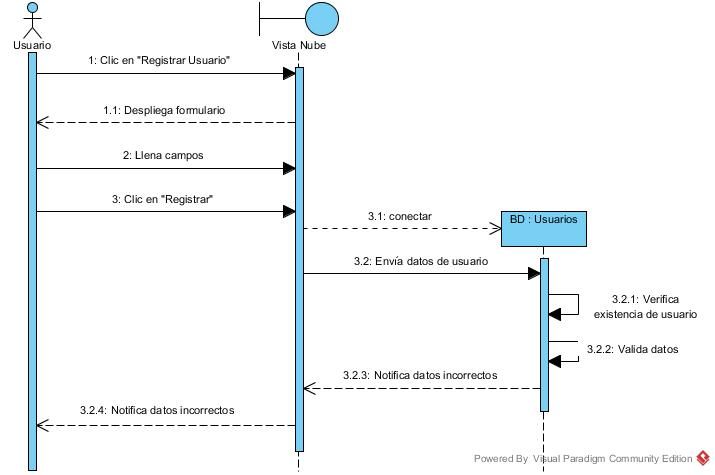
\includegraphics[width=1\textwidth]{images/Registrar_trayectoria_a}
\caption{Diagrama de secuencias de Registrar un usuario nuevo con datos incorrectos.}
\end{figure}

\begin{figure}[htbp!]
\centering
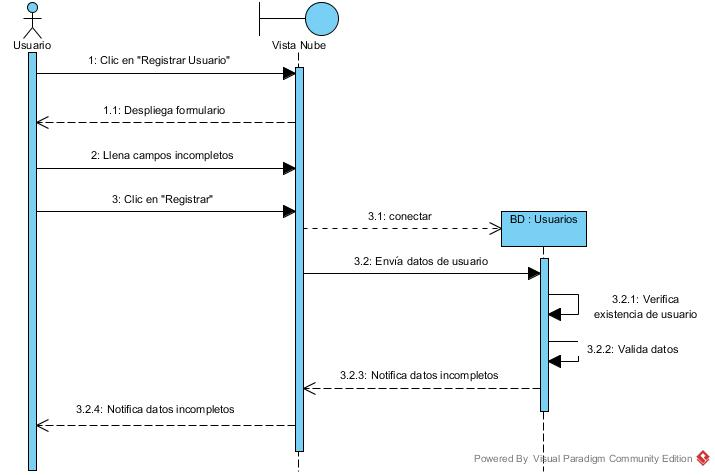
\includegraphics[width=1\textwidth]{images/Registrar_trayectoria_b}
\caption{Diagrama de secuencias de Registrar un usuario nuevo con datos incompletos.}
\end{figure}

\begin{figure}[htbp!]
\centering
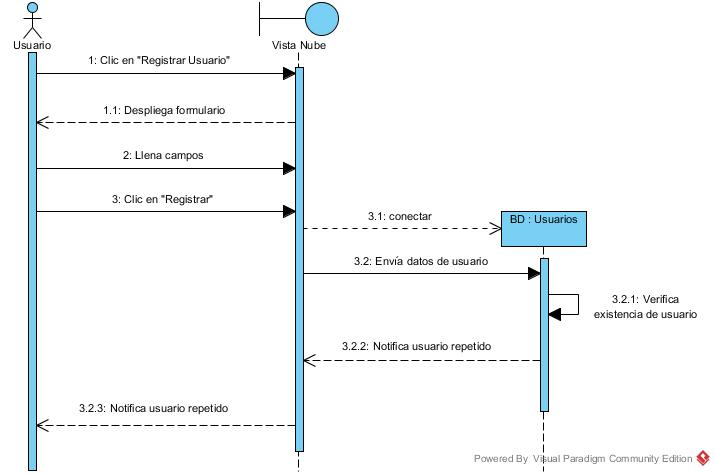
\includegraphics[width=1\textwidth]{images/Registrar_trayectoria_c}
\caption{Diagrama de secuencias de Registrar un usuario nuevo con usuario repetido.}
\end{figure} 
\newpage

\subsection{Iniciar Sesión}

\begin{figure}[htbp!]
\centering
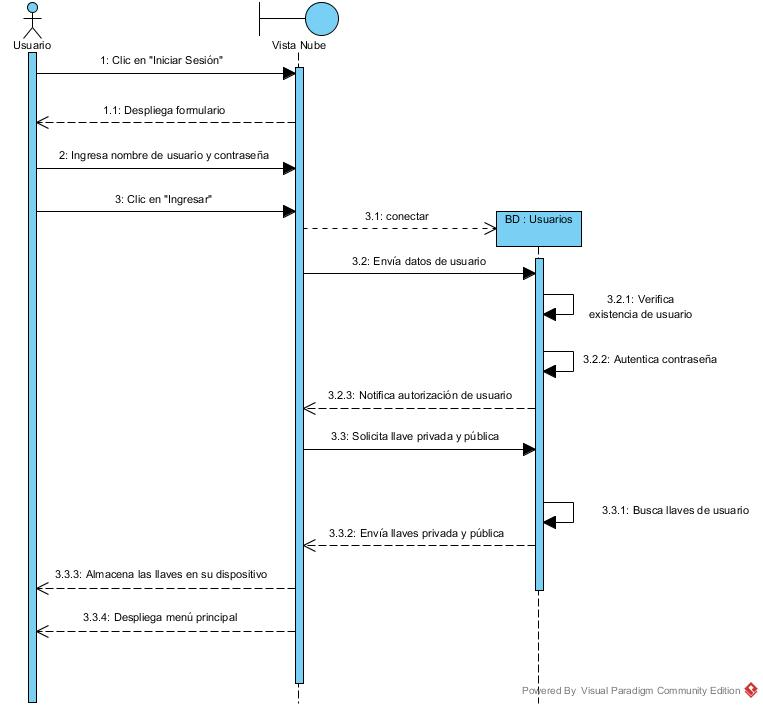
\includegraphics[width=1\textwidth]{images/Iniciar_sesion}
\caption{Diagrama de secuencias de Iniciar sesión un usuario.}
\end{figure}

\begin{figure}[htbp!]
\centering
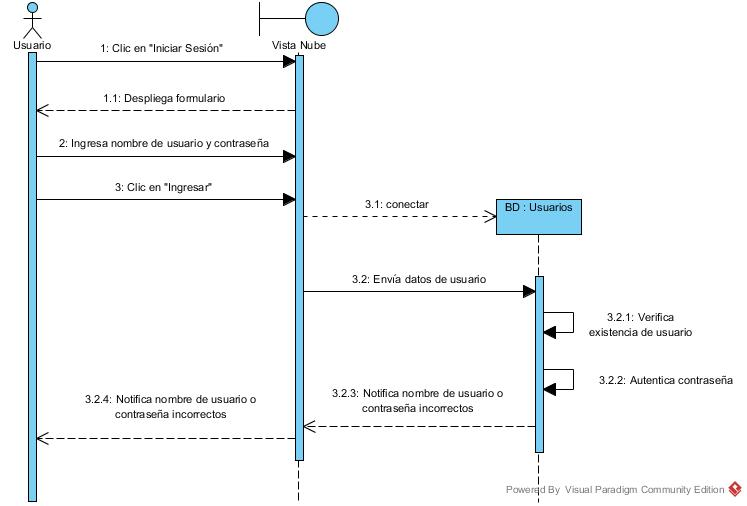
\includegraphics[width=1\textwidth]{images/Iniciar_trayectoria_a}
\caption{Diagrama de secuencias de Iniciar sesión un usuario con datos incorrectos.}
\end{figure}

\begin{figure}[htbp!]
\centering
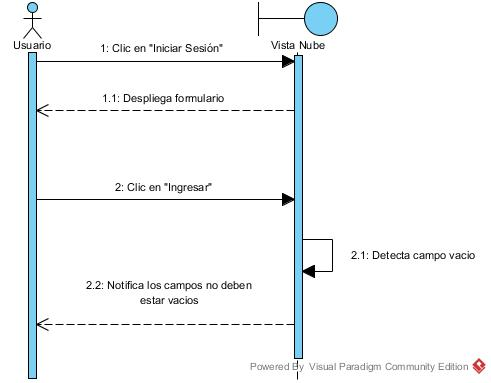
\includegraphics[width=1\textwidth]{images/Iniciar_trayectoria_b}
\caption{Diagrama de secuencias de Registrar un usuario nuevo con datos incompletos.}
\end{figure}

\begin{figure}[htbp!]
\centering
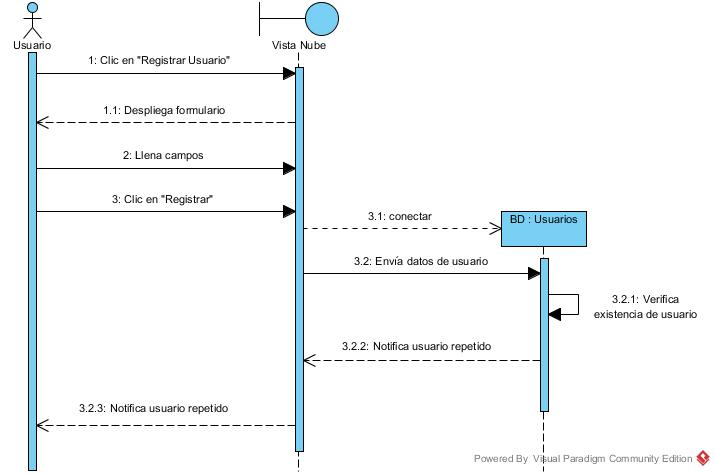
\includegraphics[width=1\textwidth]{images/Registrar_trayectoria_c}
\caption{Diagrama de secuencias de Iniciar sesión un usuario con campos vacíos.}
\end{figure} 
\newpage

\subsection{Subir Archivo}

\begin{figure}[htbp!]
\centering
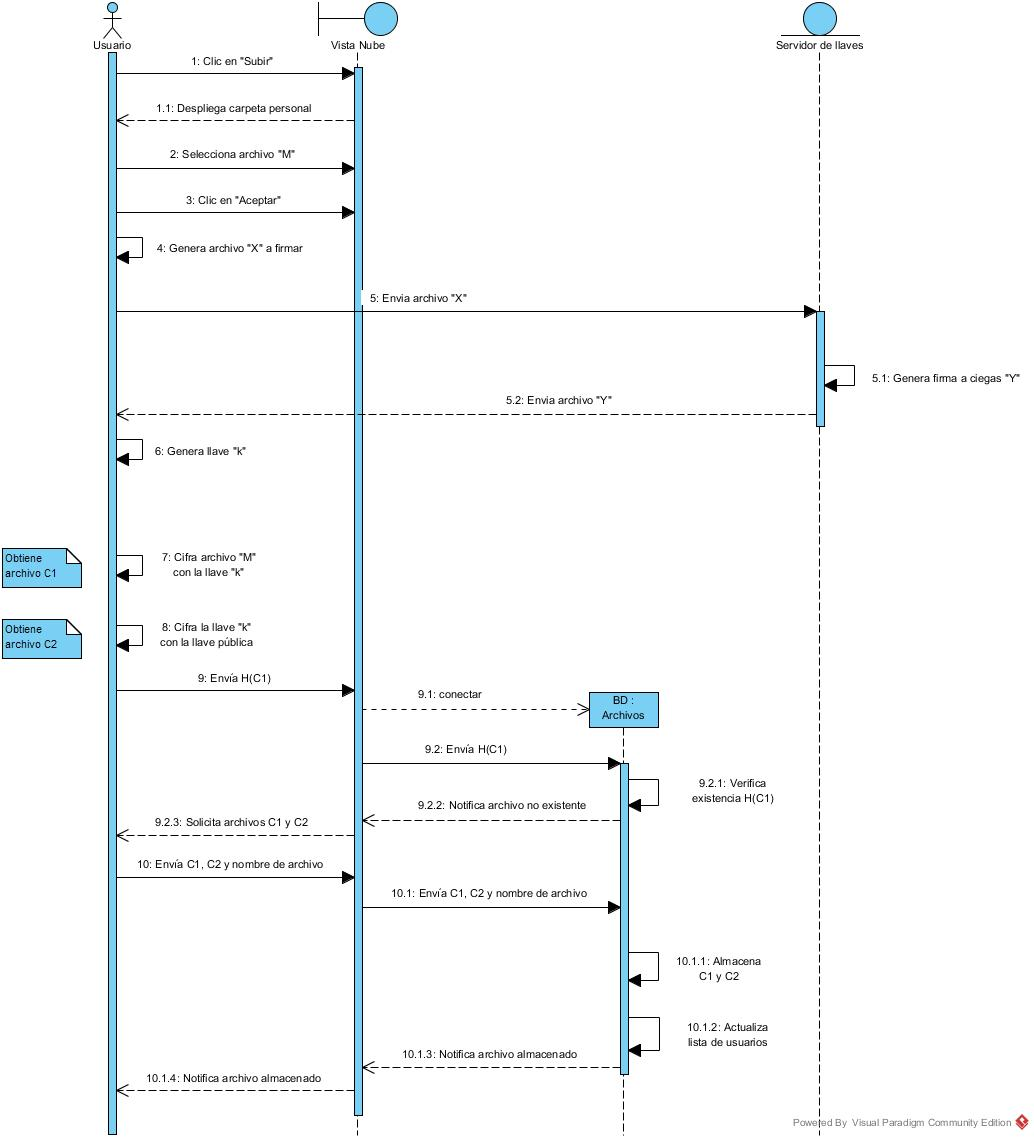
\includegraphics[width=1\textwidth]{images/Subir_Archivo}
\caption{Diagrama de secuencias de subir un archivo nuevo.}
\end{figure}

\begin{figure}[htbp!]
\centering
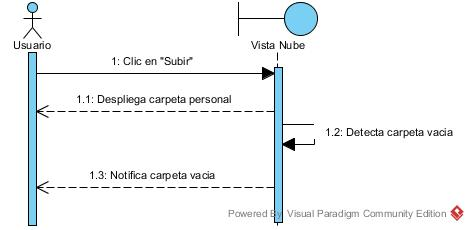
\includegraphics[width=1\textwidth]{images/Subir_trayectoria_a}
\caption{Diagrama de secuencias de subir un archivo con carpeta vacía.}
\end{figure}

\begin{figure}[htbp!]
\centering
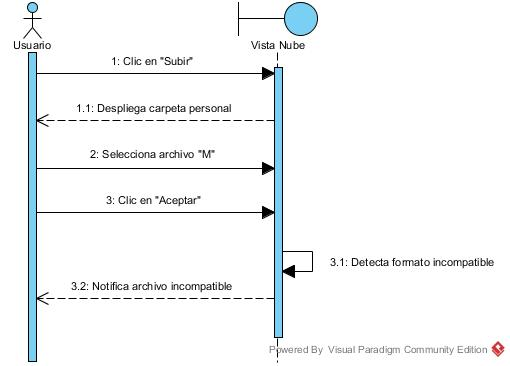
\includegraphics[width=1\textwidth]{images/Subir_trayectoria_b}
\caption{Diagrama de secuencias de subir un archivo incompatible.}
\end{figure}

\begin{figure}[htbp!]
\centering
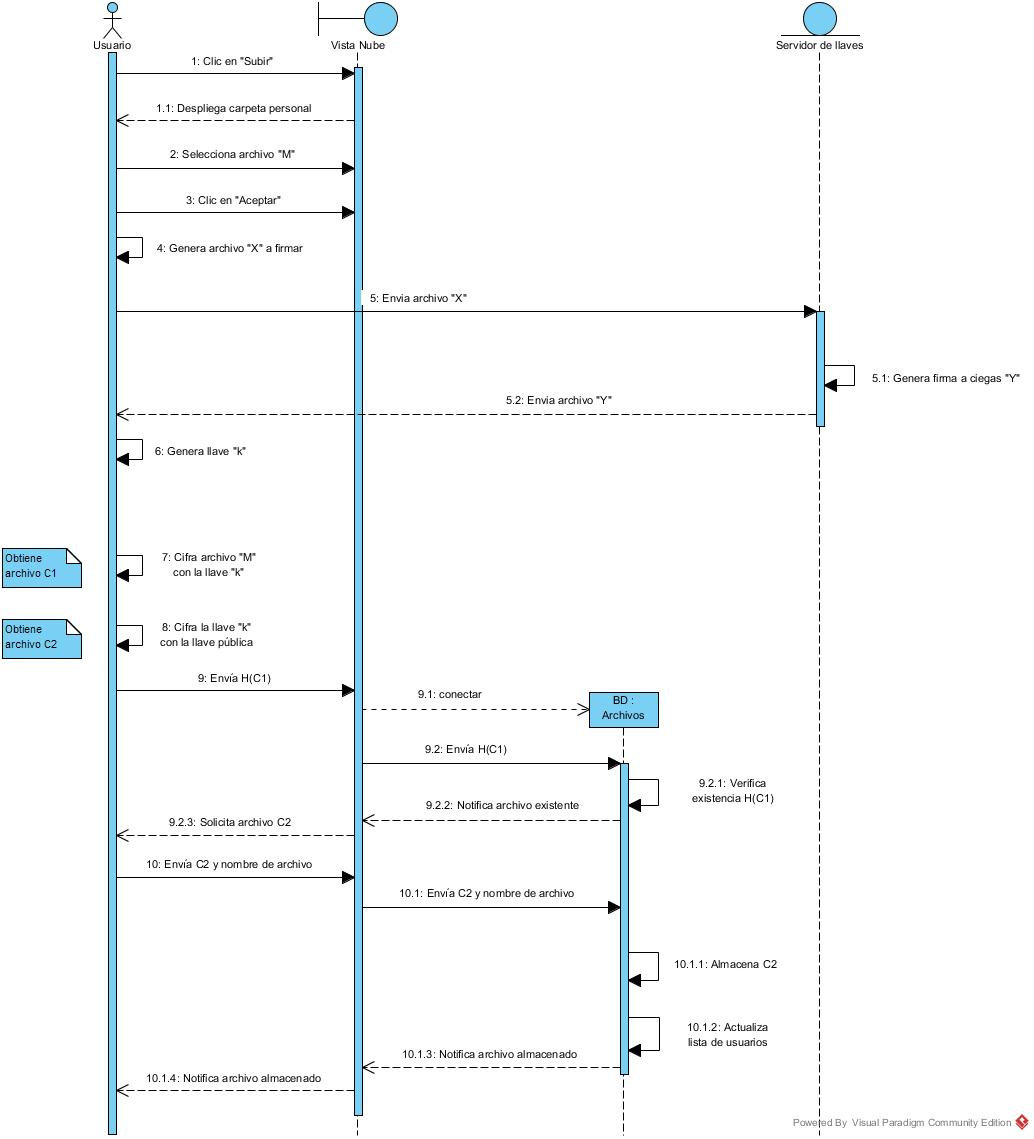
\includegraphics[width=1\textwidth]{images/Subir_trayectoria_c}
\caption{Diagrama de secuencias de subir un archivo existente.}
\end{figure} 
\newpage

\subsection{Firma a ciegas}

\begin{figure}[htbp!]
\centering
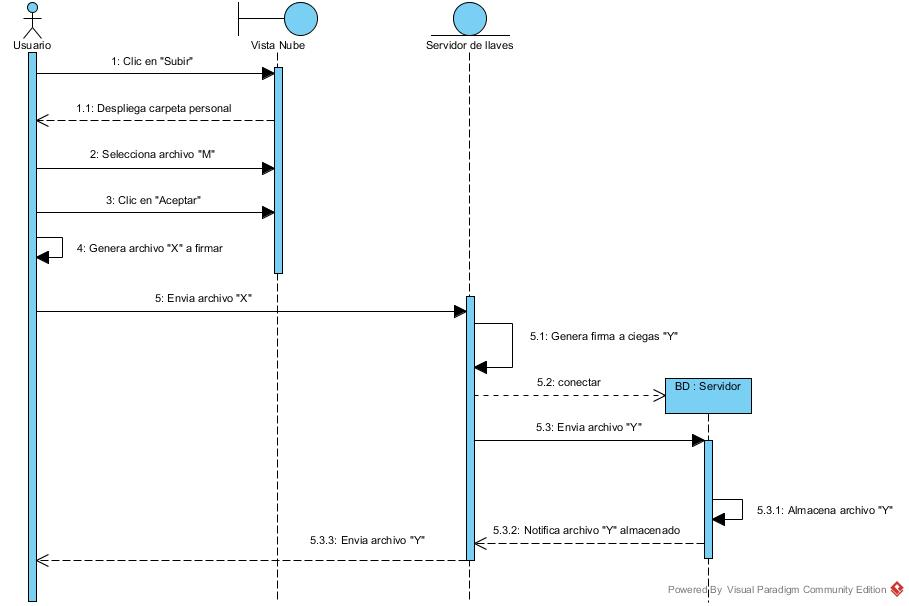
\includegraphics[width=1\textwidth]{images/Firma_ciegas}
\caption{Diagrama de secuencias de la firma a ciegas del servidor de llaves.}
\end{figure} 
\newpage

\subsection{Descargar Archivo}

\begin{figure}[htbp!]
\centering
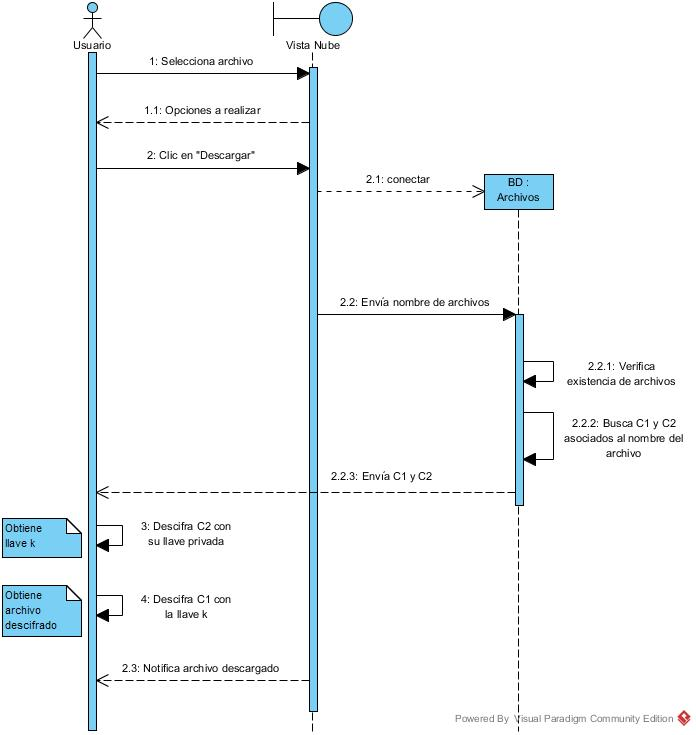
\includegraphics[width=1\textwidth]{images/Descargar_Archivo}
\caption{Diagrama de secuencias de descargar un archivo de la nube.}
\end{figure}

\begin{figure}[htbp!]
\centering
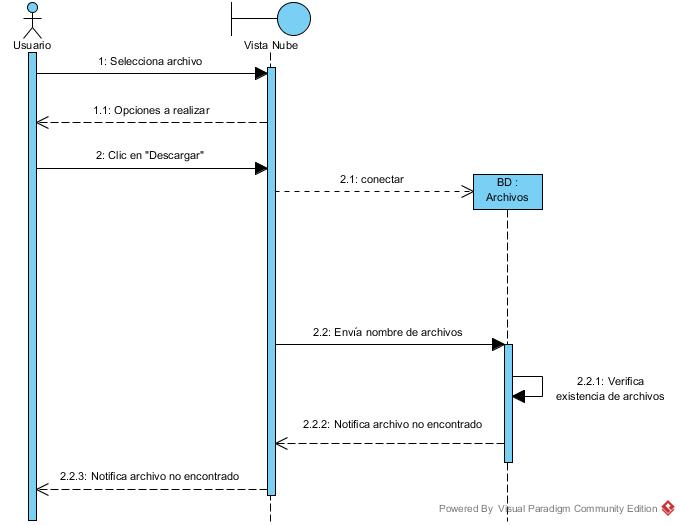
\includegraphics[width=1\textwidth]{images/Descargar_aleternativa_a}
\caption{Diagrama de secuencias de descargar un archivo de la nube no encontrado.}
\end{figure} 
\newpage

\subsection{Eliminar Archivo}

\begin{figure}[htbp!]
\centering
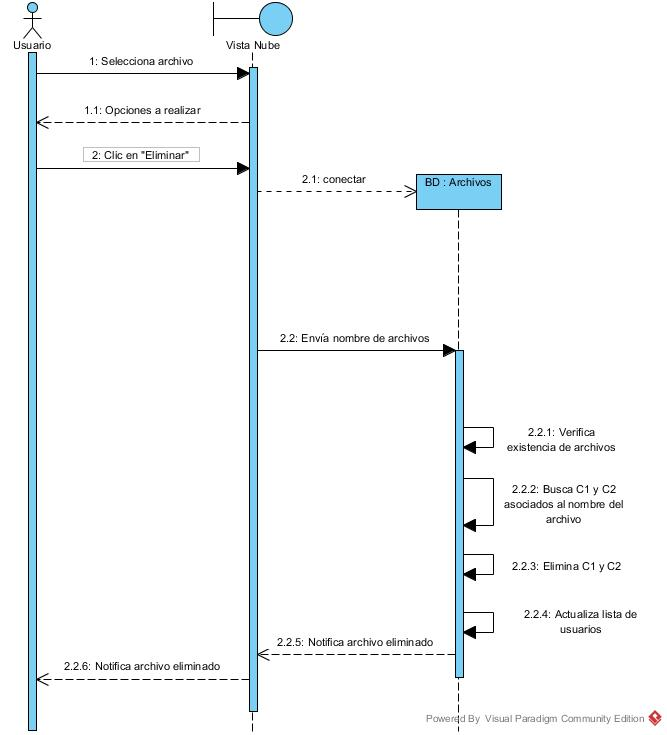
\includegraphics[width=1\textwidth]{images/Eliminar_Archivo}
\caption{Diagrama de secuencias de eliminar un archivo de la nube.}
\end{figure} 
\newpage

%=======================================================================================================================================
\cfinput{casosUso/Mensajes/mensajes}
